% !TeX document-id = {31322199-07d0-4e7b-ac39-8f4bff032313}
% !TeX root = workshop-codemash-2023.tex
% !TeX TXS-program:compile = txs:///pdflatex/[--shell-escape]
% !TeX encoding = UTF-8
% !TeX spellcheck = en_US
% https://orcid.org/0000-0003-4586-8500
% session details: https://www.codemash.org/session-details/?id=375030

% Other possible values are: 1610, 149, 54, 43 and 32.
% By default, it is to 128mm by 96mm(4:3)
\documentclass[aspectratio=169]{beamer}

%\setbeamertemplate{headline navigation symbols}{}         % no navigation symbols
\usetheme{Warsaw}
\usecolortheme{seahorse}
\usepackage[absolute,overlay]{textpos} % Text positioning

%%%%%%%%%%%%%%%%%%% TEXT COLOR %%%%%%%%%%%%%%%%%
\usepackage{xcolor}
\definecolor{olive}{rgb}{0.3, 0.4, .1}
\definecolor{fore}{RGB}{249,242,215}
\definecolor{back}{RGB}{51,51,51}
\definecolor{title}{RGB}{255,0,90}
\definecolor{dgreen}{rgb}{0.,0.6,0.}
\definecolor{gold}{rgb}{1.,0.84,0.}
\definecolor{JungleGreen}{cmyk}{0.99,0,0.52,0}
\definecolor{BlueGreen}{cmyk}{0.85,0,0.33,0}
\definecolor{RawSienna}{cmyk}{0,0.72,1,0.45}
\definecolor{Magenta}{cmyk}{0,1,0,0}

%Information to be included in the title page:
\title{Build a Serverless Github Bot in GCP}
\subtitle{}
\author{Franklin Diaz}
\institute{DE:AD:10:C5}
\date{Tuesday January 10, 2023}


\begin{document}

%%% Title Slide %%%
\frame{\titlepage}


%\begin{frame}
%        \frametitle{Table of Contents}
%        \tableofcontents
%\end{frame}

% uncomment one of these for the whole doc, or add at the start of a section as desired                                                                 
%\usebackgroundtemplate{
\includegraphics[width=\paperwidth]{../images/field.jpg}}
\usebackgroundtemplate{
\includegraphics[width=\paperwidth]{../images/landscape.jpg}}
%\usebackgroundtemplate{
\includegraphics[width=\paperwidth]{../images/tree.jpg}}


\section{INTRODUCTION}
\begin{frame}
	\Huge \textcolor{dgreen}{INTRODUCTION}
\end{frame}

% you can uncomment one of these for the whole doc, or add at the start of each section as desired                                                                            
\usebackgroundtemplate{
\includegraphics[width=\paperwidth]{../images/field.jpg}}
%\usebackgroundtemplate{
\includegraphics[width=\paperwidth]{../images/landscape.jpg}}
%\usebackgroundtemplate{
\includegraphics[width=\paperwidth]{../images/tree.jpg}}

\begin{frame}
	\frametitle{Overview: Usage}
	The big picture for operation.
	\vspace{2mm}

	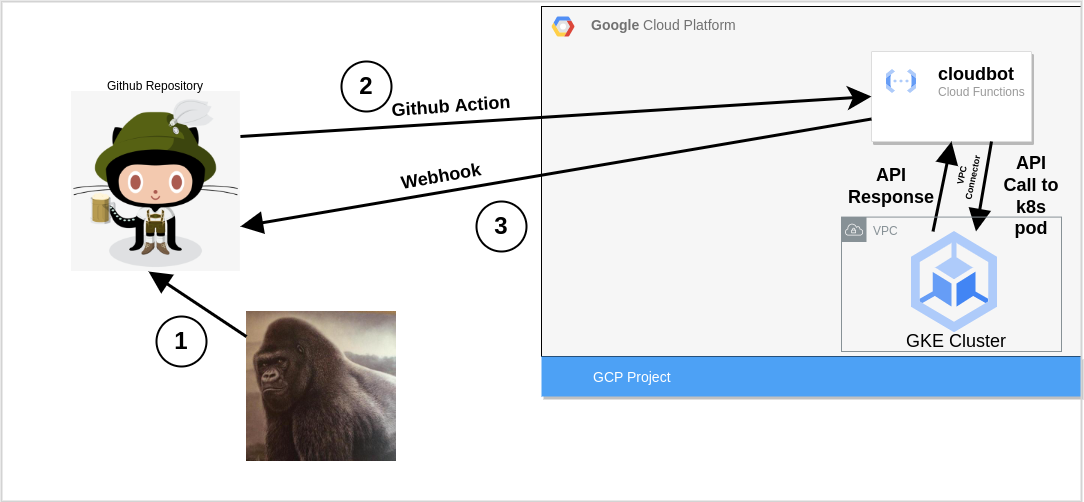
\includegraphics[width=0.785\textwidth]{../images/arch_diagrams-big-block.png}

\end{frame}

\note[itemize]{
	\item Notice that a full working version of this project is running on the Github repository for the project.
	\item In the first step, you push a code change to your github repository.
	\item In step 2, a GH action triggers a call to the the cloud function in GCP.
	\item In step 3, the cloud function makes a call to the webhook in Github.
}

\begin{frame}
	\frametitle{Overview: Deployment}
	The big picture for deployment.
	\vspace{2mm}
\end{frame}

\note[itemize]{
	\item Need a diagram that shows the flow of the application deployment.
}

\begin{frame}
	\frametitle{Outline}
	A high level overview of the learning path is as follows:
	\begin{raggedright}
		\begin{itemize}
			\item Prerequisites
			\item Github setup.
			\item Set up a development environment.
			\item Review the Python source for the bot.
			\item Configure Terraform and deploy the bot.
			\item Test it out.
			\item Explore possibilities for extending the functionality.
		\end{itemize}
	\end{raggedright}
	\vspace{2mm}
\end{frame}

% uncomment one of these for the whole doc, or add at the start of a section as desired                                                                 
%\usebackgroundtemplate{
\includegraphics[width=\paperwidth]{../images/field.jpg}}
\usebackgroundtemplate{
\includegraphics[width=\paperwidth]{../images/landscape.jpg}}
%\usebackgroundtemplate{
\includegraphics[width=\paperwidth]{../images/tree.jpg}}


\section{PRE-WORK}
\begin{frame}
	\Huge \textcolor{dgreen}{PRE-WORK}
\end{frame}

% you can uncomment one of these for the whole doc, or add at the start of each section as desired                                                                            
\usebackgroundtemplate{
\includegraphics[width=\paperwidth]{../images/field.jpg}}
%\usebackgroundtemplate{
\includegraphics[width=\paperwidth]{../images/landscape.jpg}}
%\usebackgroundtemplate{
\includegraphics[width=\paperwidth]{../images/tree.jpg}}

\begin{frame}
	\frametitle{Setup: VSCode}
	VSCode (\href{https://code.visualstudio.com}{https://code.visualstudio.com})
	\begin{itemize}
		\item Windows 64 bit User Installer: \href{https://prereqs.codemash.org/Files/VVSCodeUserSetup-x64-1.73.1.exe}{VSCodeUserSetup-x64-1.73.1.exe}
		\item Mac Universal: \href{https://prereqs.codemash.org/Files/VSCode-darwin-universal.zip}{VSCode-darwin-universal.zip}
		\item Linux (Debian, Ubuntu): \href{https://prereqs.codemash.org/Files/code_1.73.1-1667967334_amd64.deb}{code\_1.73.1-1667967334\_amd64.deb}
		\item  Linux (Red Hat, Fedora, SUSE): \href{https://prereqs.codemash.org/Files/code-1.73.1-1667967421.el7.x86_64.rpm}{code-1.73.1-1667967421.el7.x86\_64.rpm}
	\end{itemize}
	\vspace{2mm}
	\href{https://code.visualstudio.com/docs/devcontainers/containers}{Click this link for details on using dev containers in VSCode}
\end{frame}

\begin{frame}
	\frametitle{Setup: git}
	GIT (\href{https://git-scm.com/downloads}{https://git-scm.com/downloads})
	\begin{itemize}
		\item Windows 32 Bit: \href{https://prereqs.codemash.org/Files/Git-2.38.1-64-bit.exe}{Git-2.38.1-64-bit.exe}
		\item Windows 64 Bit: \href{https://prereqs.codemash.org/Files/Git-2.38.1-32-bit.exe}{Git-2.38.1-32-bit.exe}
		\item Mac: \href{https://prereqs.codemash.org/Files/git-2.15.0-intel-universal-mavericks.dmg}{git-2.15.0-intel-universal-mavericks.dmg}
	\end{itemize}
\end{frame}

\begin{frame}
	\frametitle{Setup: Docker Desktop}
	Docker Desktop (\href{https://www.docker.com/}{https://www.docker.com/})

	\begin{itemize}
		\item Windows: \href{https://prereqs.codemash.org/Files/Docker\%20Desktop\%20Installer.exe}{Docker Desktop Installer.exe}
		\item MacOS (Intel Chip): \href{https://prereqs.codemash.org/Files/Docker.dmg}{Docker.dmg}
		\item MacOS (M1 Chip): \href{https://prereqs.codemash.org/Files/Chip/Docker.dmg}{Docker.dmg}
		\item Linux instructions can be found: \href{https://docs.docker.com/desktop/install/linux-install/}{here}
	\end{itemize}
	\vspace{2mm}

	\href{https://code.visualstudio.com/docs/devcontainers/containers\#\_installation}{Click here to see Docker setup steps from Microsoft}

\end{frame}

\note[itemize]{
	\item this is a test
}

\begin{frame}
	\frametitle{Setup: Clone and Open the Project Repository}
	\begin{itemize}
		\item Time to clone the repository.
		\item \href{https://github.com/devsecfranklin/workshop-codemash-2023}{Click this link for the Github repository}
		\item In VSCode, press F1 and enter the command ``Dev Containers: Open Folder in Container''
		\begin{itemize}
			\item You can also choose ``Dev Containers: Open Workspace in Container''
			\item \href{https://code.visualstudio.com/docs/devcontainers/tutorial}{Here is the Microsoft VSCode dev containers tutorial}
		\end{itemize}
		\item From the top menu select ``Terminal -- New Terminal''
		\item Now ``cd /workspaces/workshop-codemash-2023/bin'' and type ``setup-dev-env.sh''
	\end{itemize}
	\vspace{2mm}
\end{frame}

\note[itemize]{
	\item this is a test
}

\begin{frame}
	\frametitle{Google Cloud: Account Setup}
	\begin{itemize}
		\item \href{https://cloud.google.com/free}{Sign up for a free tier GCP account}.
		\item Navigate to \href{https://cloud.google.com/}{https://cloud.google.com/} and make sure you have a usable project to work in.
		\item \href{https://cloud.google.com/resource-manager/docs/creating-managing-projects}{Here is some infomration about creating projects in GCP}
	\end{itemize}
\end{frame}

% uncomment one of these for the whole doc, or add at the start of a section as desired                                                                 
%\usebackgroundtemplate{
\includegraphics[width=\paperwidth]{../images/field.jpg}}
\usebackgroundtemplate{
\includegraphics[width=\paperwidth]{../images/landscape.jpg}}
%\usebackgroundtemplate{
\includegraphics[width=\paperwidth]{../images/tree.jpg}}

\section{IN CLASS SETUP}
\begin{frame}
	\Huge \textcolor{dgreen}{IN CLASS SETUP}
\end{frame}

% you can uncomment one of these for the whole doc, or add at the start of each section as desired                                                                            
\usebackgroundtemplate{
\includegraphics[width=\paperwidth]{../images/field.jpg}}
%\usebackgroundtemplate{
\includegraphics[width=\paperwidth]{../images/landscape.jpg}}
%\usebackgroundtemplate{
\includegraphics[width=\paperwidth]{../images/tree.jpg}}

\begin{frame}
	\frametitle{Google Cloud: Update Project Name and Login}
	\begin{itemize}
		\item Update your project name in the file ``/workspaces/workshop-codemash-2023/.envrc''
		\item Update your project name in the file ``/workspaces/workshop-codemash-2023/src/config.ini''
		\item Type the command ``direnv allow .'' to reload the ENV variables.
		\item In the dev container, run the command ``gcloud auth login'' and follow the directions there.
		\item Verify you are connected to GCP with the command ``gcloud auth list''	
	\end{itemize}
\end{frame}

\begin{frame}
	\frametitle{Google Cloud: Create Service User}
	
	We create a service user in GCP with limited scope of permissions.
	
\end{frame}

\begin{frame}
	\frametitle{Google Cloud: Create Secret in Secrets Mgr}
	
	\begin{itemize}
		\item The Cloud Function is expecting us to create a secret named ``gh\_secret\_token''.
	\end{itemize}
	
\end{frame}

% uncomment one of these for the whole doc, or add at the start of a section as desired                                                                 
%\usebackgroundtemplate{
\includegraphics[width=\paperwidth]{../images/field.jpg}}
\usebackgroundtemplate{
\includegraphics[width=\paperwidth]{../images/landscape.jpg}}
%\usebackgroundtemplate{
\includegraphics[width=\paperwidth]{../images/tree.jpg}}


\section{PYTHON}
\begin{frame}
	\Huge \textcolor{dgreen}{PYTHON}
\end{frame}

% you can uncomment one of these for the whole doc, or add at the start of each section as desired                                                                            
\usebackgroundtemplate{
\includegraphics[width=\paperwidth]{../images/field.jpg}}
%\usebackgroundtemplate{
\includegraphics[width=\paperwidth]{../images/landscape.jpg}}
%\usebackgroundtemplate{
\includegraphics[width=\paperwidth]{../images/tree.jpg}}

\begin{frame}
	\frametitle{Overview: Python Functions}
	The big picture for the Python code files.
	\vspace{2mm}
	
	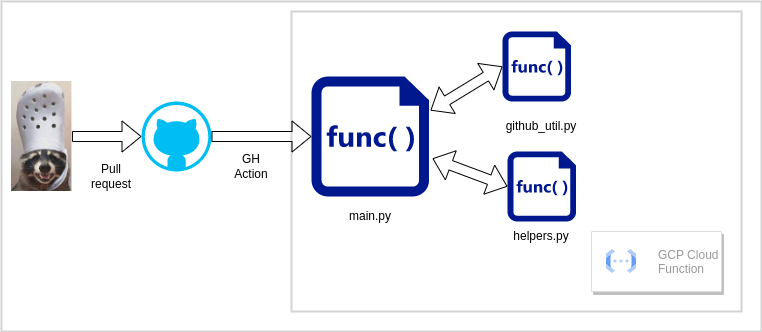
\includegraphics[width=0.785\textwidth]{../images/arch_diagrams-python-big-block.png}
\end{frame}
\note[itemize]{
	\item Note that there are three Python files.
	\item the main.py file is called via Github action.
	\item the other two files have functions to help us manage the pull request.
}

\begin{frame}
	\frametitle{The Python Application}

	Discuss the code for the cloud function, see how all that works.

\end{frame}

\note[itemize]{
	\item Need a diagram that shows the flow in the Python files.
}


% uncomment one of these for the whole doc, or add at the start of a section as desired                                                                 
%\usebackgroundtemplate{
\includegraphics[width=\paperwidth]{../images/field.jpg}}
\usebackgroundtemplate{
\includegraphics[width=\paperwidth]{../images/landscape.jpg}}
%\usebackgroundtemplate{
\includegraphics[width=\paperwidth]{../images/tree.jpg}}


\section{TERRAFORM}
\begin{frame}
	\Huge \textcolor{dgreen}{TERRAFORM}
\end{frame}

% you can uncomment one of these for the whole doc, or add at the start of each section as desired                                                                            
\usebackgroundtemplate{
\includegraphics[width=\paperwidth]{../images/field.jpg}}
%\usebackgroundtemplate{
\includegraphics[width=\paperwidth]{../images/landscape.jpg}}
%\usebackgroundtemplate{
\includegraphics[width=\paperwidth]{../images/tree.jpg}}

\begin{frame}
	\frametitle{The Terraform Installer}

	We use Terraform to automate the Cloud Function installation.

\end{frame}

\begin{frame}
	\frametitle{Deploying with Terraform}

	Let's do a Terraform deployment.

\end{frame}

% uncomment one of these for the whole doc, or add at the start of a section as desired                                                                 
%\usebackgroundtemplate{
\includegraphics[width=\paperwidth]{../images/field.jpg}}
\usebackgroundtemplate{
\includegraphics[width=\paperwidth]{../images/landscape.jpg}}
%\usebackgroundtemplate{
\includegraphics[width=\paperwidth]{../images/tree.jpg}}


\section{EXTRA}
\begin{frame}
	\Huge \textcolor{dgreen}{EXTRA}
\end{frame}

% you can uncomment one of these for the whole doc, or add at the start of each section as desired                                                                            
\usebackgroundtemplate{
\includegraphics[width=\paperwidth]{../images/field.jpg}}
%\usebackgroundtemplate{
\includegraphics[width=\paperwidth]{../images/landscape.jpg}}
%\usebackgroundtemplate{
\includegraphics[width=\paperwidth]{../images/tree.jpg}}

\begin{frame}
	\frametitle{Extra: Dockerfile and docker-compose.yml}

	Check out the docker container and framework, see how all that works.

\end{frame}


\begin{frame}
	\frametitle{Extra: Connect it to your GKE cluster}

	I can demo this or we can try it if we have time.

\end{frame}

\begin{frame}
	\frametitle{Extra: GNU Autotools}

	Wow we must be super bored let\'s play with GNU Autotools.

\end{frame}

\begin{frame}
	\frametitle{Future: Scan the PR comments for commands}

	The Cloud Function could monitor the PR for certain strings, using these to trigger actions.

\end{frame}

\begin{frame}
	\frametitle{Resources}
	\href{https://www.codemash.org/session-details/?id=375030}{Click here for Session Details}
	\vspace{2mm}

	Project source files are available: \url{https://github.com/devsecfranklin/workshop-codemash-2023}
	\vspace{2mm}

	Prerequisites are \href{https://prereqs.codemash.org/}{available at this link}.
\end{frame}

\begin{frame}
	\frametitle{Contact}
	\begin{columns}
		\begin{column}{0.5\textwidth}
			Mastodon: ``@devsecfranklin@defcon.social''
			\vspace{2mm}

			E-mail: \textbf{\href{mailto:devsecfranklin@duck.com}{devsecfranklin@duck.com}}
		\end{column}
		\begin{column}{0.5\textwidth}
			\begin{center}
				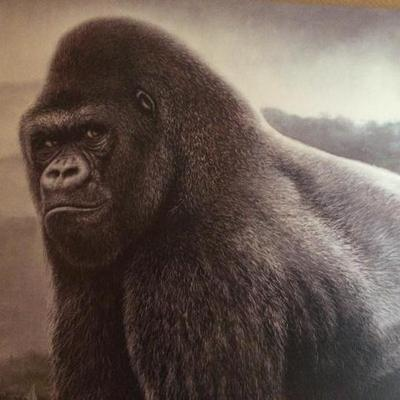
\includegraphics[width=0.785\textwidth]{../images/rilla.jpg}
			\end{center}
		\end{column}
	\end{columns}
\end{frame}

\end{document}